\chapter{Метод нечеткого вывода на основе нечеткого значения истинности}\label{ch:ch2}

\section{Постановка задачи нечеткого вывода}\label{sec:ch2/fuzzy-inference-problem-statement}

Лингвистическая модель представляет собой базу правил вида:
\begin{equation}
\label{eqn:fuz-problem-1}
R_k:\ \text{Если}\ x_1\ \text{есть}\ A_{k1}\ \text{и}\ x_2\ \text{есть}\ A_{k2}\ \text{и} \dots \text{и}\ x_n\ \text{есть}\ A_{kn}, \text{то}\ y\ \text{есть}\ B_k,
\end{equation}
где $N$ "--- количество нечетких правил, $A_{ki} \subseteq X_i, i=\overline{1,n}, B_k \subseteq Y$"--- нечеткие множества, которые характеризуются функциями принадлежности $\mu_{A_{ki}}(x_i)$ и $\mu_{B_k}(y)$ соответственно; $x_1, x_2,…,x_n$"--- входные переменные лингвистической модели, причем
\[
[x_1, x_2, ..., x_n]^T = \mathbf{x} \in X_1 \times X_2 \times \dots \times X_n.
\]

Символами  $X_i, i=\overline{1,n}$ и $Y$ обозначаются соответственно пространства входных и выходной переменных. Если ввести обозначения $\mathbf{X}=X_1 \times X_2 \times \dots \times X_n$ и $\mathbf{A_k}=A_{k1}\times A_{k2} \times \dots \times A_{kn}$ , причем
\[
\mu_\mathbf{A_k}(\mathbf{x}) = \underset{i=\overline{1,n}}{T_1} \mu_{A_{ki}}(x_i),
\]
где $T_1$ - произвольная $t$-норма, то правило \ref{eqn:2.1} представляется в виде нечеткой импликации
\begin{equation}
\label{eqn:fuz-problem-2}
R_k: \mathbf{A_k} \to B_k, k=\overline{1,N}.
\end{equation}

Правило $R_k$ можно формализовать как нечеткое отношение, определенное на множестве  $\mathbf{X}\times Y$, т.е. $R_k \subseteq \mathbf{X} \times Y$ - нечеткое множество с функцией принадлежности
\[
\mu_{R_k}(\mathbf{x}, y) = \mu_{\mathbf{A_k} \to B_k} (\mathbf{x}, y).
\]

Модель логического типа определяет задание функции $\mu_{\mathbf{A_k} \to B_k} (\mathbf{x}, y)$ на основе известных функций принадлежности $\mu_{\mathbf{A_k}}(\mathbf{x})$ и $\mu_{B_k}(y)$ с помощью одной из предложенных в [2] функций импликации:
\[
\mu_{\mathbf{A_k} \to B_k} (\mathbf{x}, y) = I(\mu_{\mathbf{A_k}}(\mathbf{x}), \mu_{B_k}(y)),
\]
где $I$"--- некоторая импликация.

Ставится задача определить нечеткий вывод $B'_k \subseteq Y$ для системы, представленной в виде (\ref{eqn:2.1}), если на входах - нечеткие множества.
$\mathbf{A'}=A'_1 \times A'_2 \times \dots \times A'_n \subseteq \mathbf{X}$ или $x_1\ \text{есть}\ A'_1\ \text{и}\ x_2\ \text{есть}\ A'_2\ \text{и} \dots \text{и}\ x_n\ \text{есть}\ A'_n$  с соответствующей функцией принадлежности $\mu_{\mathbf{A'}}(\mathbf{x})$, которая определяется как
\begin{equation}
\label{eqn:fuz-problem-3}
\mu_{\mathbf{A'}}(\mathbf{x}) = \underset{i=\overline{1,n}}{T_3} \mu_{A'_i}(x_i).
\end{equation}

Несинглтонный фаззификатор отображает измеренное $x_i=x'_i, i=\overline{1,n}$ в нечеткое число, для которого $\mu_{A'_i}(x'_i) = 1$ и $\mu_{A'_i}(x_i)$ уменьшается от единицы по мере удаления от  $x'_i$.
В соответствии с обобщенным нечетким правилом modus ponens [2], нечеткое множество $B'_k$ определяется композицией нечеткого множества $\mathbf{A'}$ и отношения $\mathbf{R_k}$, т.е.
\[
B'_k = \mathbf{A'} \circ (\mathbf{A_k} \to B_k),
\]
или, на уровне функций принадлежности
\begin{equation}
\label{eqn:fuz-problem-4}
\mu_{B'_k}(y|\mathbf{x'}) = \sup_{\mathbf{x}\in \mathbf{X}}\left\{\mu_{\mathbf{A'}}(\mathbf{x'})\overset{T_2}{\star} I(\mu_{\mathbf{A_k}}(\mathbf{x}), \mu_{B_k}(y))\right\}.
\end{equation}

В (\ref{eqn:fuz-problem-4}) применена условная нотация, так как ввод в нечеткую систему происходит при определенном значении $\mathbf{x}$, а именно $\mathbf{x'}$. Обозначение $\mu_{B'_k}(y | \mathbf{x'})$ показывает, что $\mu_{B'_k}$ изменяется с каждым значением $\mathbf{x'}$. Вычислительная сложность выражения (\ref{eqn:fuz-problem-4}) составляет $O(|X_1|\cdot |X_2|\cdot \dots \cdot |X_n|\cdot |Y|)$ т.е. экспоненциальная. 

\section{Вывод на основе нечеткого значения истинности}\label{sec:ch2/ftv-based-inference-statement}

Используя правило истинностной модификации [1] можно выразить:
\[
\mu_{A'}(\mathbf{x}) = \tau_{A|A'}(\mu_A(x))
\]
где $\tau_{A|A'}$ "--- нечеткое значение истинности (НЗИ) нечеткого множества $A$ относительно $A'$, представляющее собой функцию принадлежности совместимости $CP(A_k, A')$ $A_k$по отношению к $A'$, причем $A'$ рассматривается как достоверное [Дюбуа и др., 1990]:
\begin{equation}
\label{eqn:ftv-compute-12}
\tau_{A_k|A'}(v) = \mu_{CP(A_k, A')}(v) = \sup_{\substack{\mu_{A_k}(x) = v \\ x \in X}} \left\{ \mu_{A'}(x)\right\}.
\end{equation}

Таким образом НЗИ отражает совместимость факта с посылкой в нечеткой форме. Упрощенные подходы отображают совместимость в одно значение из диапазона впервые представленное в [5].

Перейдем от переменной $x$ к переменной $v$ в выражении нечеткого вывода (\ref{}), обозначив
\[
\mu_{A_k}(x) = v \textrm{ и } \mu_{A'}(x) = \tau_{A_k|A'}(v),
\]
то есть выполним преобразование нечетких множеств на пространстве $X$ в истинностное пространство $[0, 1]$:
\[
?????
\]

Получим:
\begin{equation}
\label{eqn:ftv-compute-4}
\mu_{A'}(x) = \tau_{A_k|A'}(\mu_{A_k}(x)) = \tau_{A_k|A'}(v)
\end{equation}

Тогда (\ref{eqn:fuz-problem-4}) примет вид:
\begin{equation}
\label{eqn:ftv-compute-5}
\mu_{B'_k}(y|\mathbf{x'}) = \sup_{v \in [0,1]}\left\{\tau_{A_k|A'}(v) \overset{T_2}{\star} I(v, \mu_{B_k}(y))\right\}.
\end{equation}

При переходе к нечеткому выводу по $n$ входам формула вычисления НЗИ для нечетких отношений посылки и факта имеет вид:
\begin{equation*}
\tau_{\mathbf{A_k}|\mathbf{A'}}(v) = \sup_{\substack{\mu_{\mathbf{A_k}}(x_1, \dots, x_n) = v \\ (x_1, \dots, x_n) \in \mathbf{x}}} \left\{\mu_{\mathbf{A'}}(x_1, \dots, x_n)\right\} .
\end{equation*}

Или в выражении через операции сверток $t$-норм $T_1$ (\ref{eqn:fuz-problem-2}) и $T_3$ (\ref{eqn:fuz-problem-3}):
\begin{equation}
\label{eqn:ftv-compute-6}
\tau_{\mathbf{A_k}|\mathbf{A'}}(v) = \sup_{\substack{\underset{i=\overline{1,n}}{\mathrm{T_1}}\mu_{A_{ki}}(x_i)=v \\ (x_1, \dots, x_n) \in \mathbf{x}}} \left\{ \underset{i=\overline{1,n}}{\mathrm{T_3}} \mu_{A'_i}(x_i) \right\}.
\end{equation}

Вместо выражения (\ref{eqn:ftv-compute-6}), НЗИ для $n$ входов может быть вычислено как свертка НЗИ по каждому отдельному входу:
\begin{equation}
\label{eqn:ftv-compute-7}
\tau_{\mathbf{A_k}|\mathbf{A'}}(v) = \underset{i=\overline{1,n}}{\mathrm{\tilde{T}}} \tau_{A_{ki}|A'_i}, v \in [0, 1],
\end{equation}
где $\mathrm{\tilde{T}}$ - расширенная по принципу обобщения $n$-местная $t$-норма \cite{kutsenko2015methods}, которая определяется как
\begin{equation}
\label{eqn:ftv-compute-8}
\underset{i=\overline{1,n}}{\mathrm{\tilde{T}}} \tau_{A_{ki}|A'_i}(v) = \sup_{\substack{\underset{i=\overline{1,n}}{\mathrm{T_1}}v_i = v \\ (v_1, \dots, v_n) \in [0, 1]^n}} \left\{\underset{i=\overline{1,n}}{\mathrm{T_3}}\tau_{A_{ki}|A'_i}(v_i)\right\}
\end{equation}
в результате перехода
\[
\mu_{A_{ki}}(x_i) = v_i \textrm{ и } \mu_{A'_i}(x_i) = \tau_{A_{ki}|A'_i}(v_i).
\]

Тогда для системы с $n$ входами выражения нечеткого вывода на основе НЗИ (\ref{eqn:ftv-compute-5}) примет вид:
\begin{equation}
\label{eqn:ftv-compute-9}
\mu_{B'_k}(y|\mathbf{x'}) = \sup_{v \in [0, 1]} \left\{\tau_{\mathbf{A_k}|\mathbf{A'}}(v) \overset{\mathrm{T_2}}{\star} I(v, \mu_{B_k}(y))\right\}
\end{equation}

Стоит отметить, что выражение (\ref{eqn:ftv-compute-7}) можно записать следующим образом, подчеркнув возможность попарного рекурсивного нахождения свертки НЗИ:
\begin{align*}
\label{eqn:ftv-compute-10}
\tau_{A_k, A'}(v) & = \underset{i=\overline{1,n}}{\mathrm{\tilde{T}_1}}\tau_{A_{ki}|A'_i}(v_i) \\
& = \left(\dots\left(\left(\mu_{CP(A_{k1}, A'_1)}(v_1)\ \mathrm{\tilde{T}_1}\ \mu_{CP(A_{k2}, A'_2)}(v_2)\right)\ \mathrm{\tilde{T}_1}\ \dots \right) \mathrm{\tilde{T}_1}\ \mu_{CP(A_{kn}, A'_n)}\right).
\end{align*}

Для $n=2$, $\mathrm{\tilde{T}}$ записывается как:
\begin{equation}
\underset{i=\overline{1,2}}{\mathrm{\tilde{T}}} \tau_{A_{ki}|A'_i}(v) = \sup_{\substack{v_1 \mathrm{ T_1 } v_2 = v \\ v_1, v_2 \in [0, 1]}} \left\{ \tau_{A_{k1}|A'_1}(v_1) \mathrm{ T_3 } \tau_{A_{k2}|A'_2}(v_2) \right\}, v \in [0,1].
\label{eqn:ftv-compute-11}
\end{equation}

При вербализации импликации в (\ref{eqn:ftv-compute-8}) она представится в виде:
\begin{equation}
\text{Если } \textit{нзи} \text{ есть } \text{ИСТИННО}, \text{ то }\ y\ \text{есть}\ B'_k
\label{eqn:ftv-compute-13}
\end{equation}

Таким образом, (\ref{eqn:ftv-compute-13}) представляет собой еще одну структуру правил в отличие от канонических структур Заде [10] и Такаги-Сугено [9]. Применение данного правила не зависит от количества входов в нечетких системах.

В формуле (\ref{eqn:ftv-compute-9}) данный подход позволяет переместить процесс вывода в единое пространство НЗИ, где функции истинности, в отличии от различных пространств в подходе Заде, могут быть объединены в более эффективный вычислительный процесс.

\begin{figure}
\centering
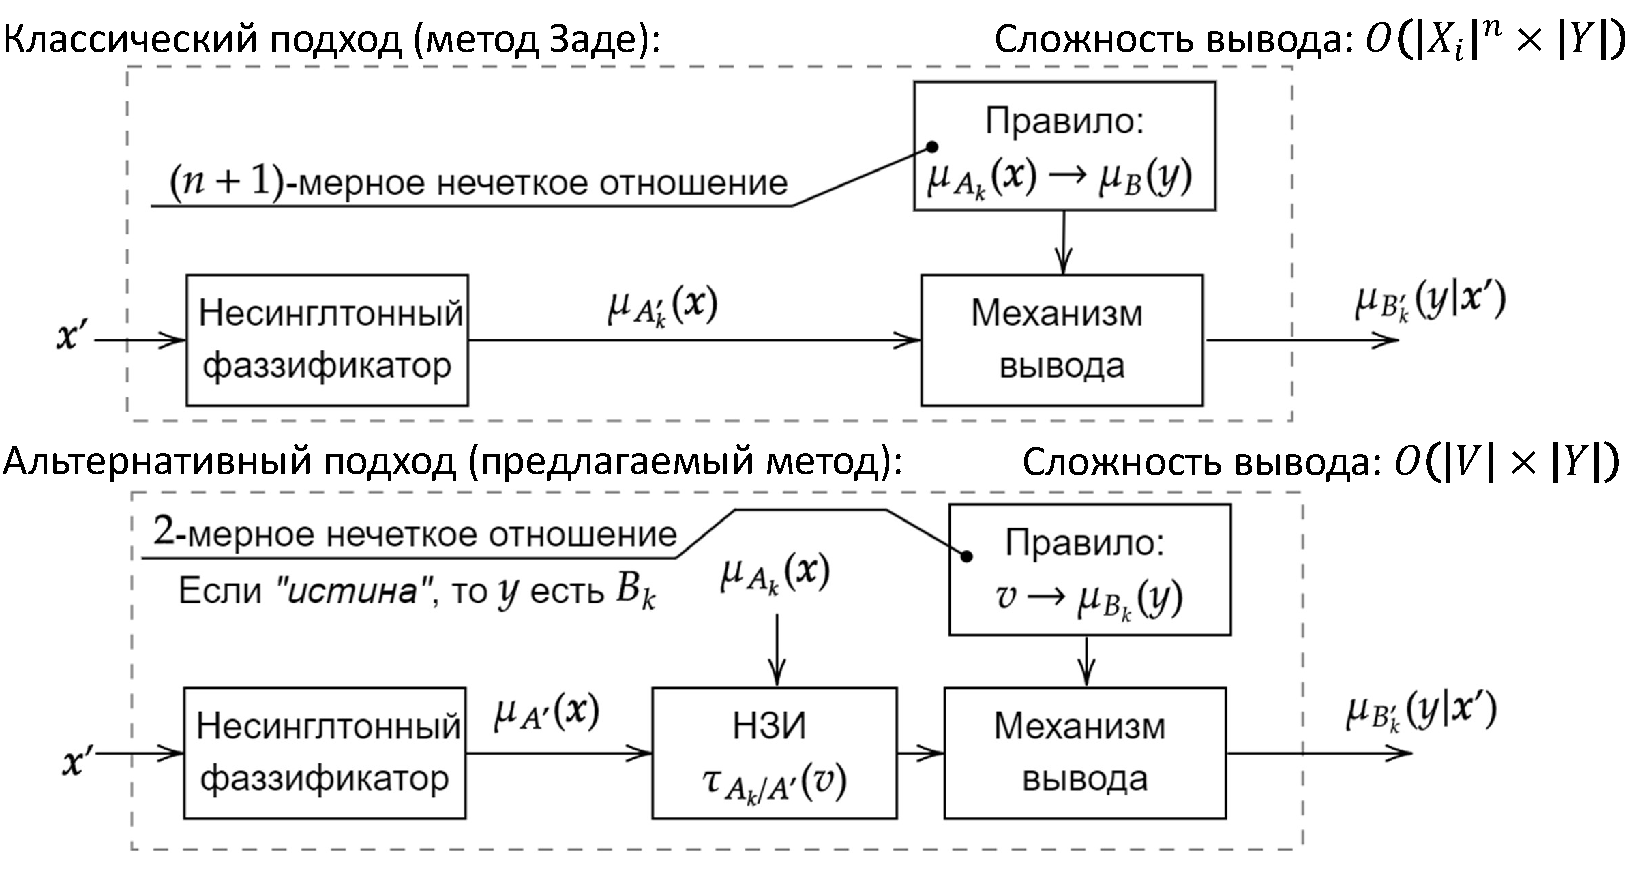
\includegraphics[scale=0.66]{ftv-schema-comparizon}
\caption{Сравнение классической схемы нечеткого вывода и схемы нечеткого вывода на основе НЗИ}
\label{fig:ftv-schema-comparizon}
\end{figure}

Порядок функции временной сложности вычисления $B'_k$ на основе выражения (\ref{eqn:ftv-compute-9}) составляет $O\left(n|V|^2+|V|\cdot |Y|\right)$, где $V=CP(A_k, A')$. Сравнение схем нечетких выводов с соответствии с соотношениями (\ref{eqn:fuz-problem-4}) и (\ref{eqn:ftv-compute-9}) представлены на рис. \cref{fig:ftv-schema-comparizon}.

\section{Вывод для систем логического типа}

\todo{\dots}
\todo{Выделяют следующие специальные категории импликаций:}
\todo{
\begin{itemize}
	\item S-импликация (Клине-Динеса, Лукасевича, Райхенбаха, Фодора): $I(a, b) = S(1-a, b)$
	\item R-импликация (Гогуен, Гедель): $I(a, b) = \sup_z \left\{z | T(a, z) \le b\right\}$
	\item Q-импликация (Заде, Вильмотта): $I(a, b) = S(1-a, T(a, b))$
\end{itemize}
}

В логическом подходе правила объединяются связкой <<И>>, тогда результирующее нечеткое множество является результатом произведения нечетких множеств, получаемых в результате нечеткого логического вывода по каждому правилу отдельно:

\begin{eqnarray}
B' = \CapOp_{r=1}^N B'_r.
\end{eqnarray}

\begin{equation}
\mu_{B'}(y) = \Tnorm_{r=1}^N \mu_{B'_r}(y) = \Tnorm_{r=1}^N \left\{\sup_{v\in [0, 1]} \left\{\tau_{A_r|A'}\overset{\mathrm{T}_2}{\star} I\left(v, \mu_{B_r}(y)\right)\right\}\right\}
\end{equation}

%Поскольку импликация в формуле (2.4)  не зависит от входных данных (\ref{eqn:2.2}), то предварительно, т.е. до использования композиционного правила (\ref{eqn:2.5}), вычисляется τ_(k,r) (v)=I(v,μ_(B_k ) (y ̅_r )) при k=(1,N) ̅,r=(1,N) ̅, v∈[0,1].



\section{Нечеткий вывод с использованием различных методов дефаззификации}

В статье \cite{VanLeekwijck1999} описывается подход к сравнению методов дефаззификации.

Описанный метод реализации \cite{eisele1994}.

\subsection{Дефаззификация по методу среднего центра}

(center average)

\begin{equation*}
	\label{eqn:defuz-ca-1}
	\hat{y}_{CA} = \frac{\sum_{k=1}^{N} \bar{y}_k \mu_{B'_k}(\bar{y}_k)}{\sum_{k=1}^{N} \mu_{B'_k}(\bar{y}_k)}
\end{equation*}

\begin{figure}[ht]
	\centering
	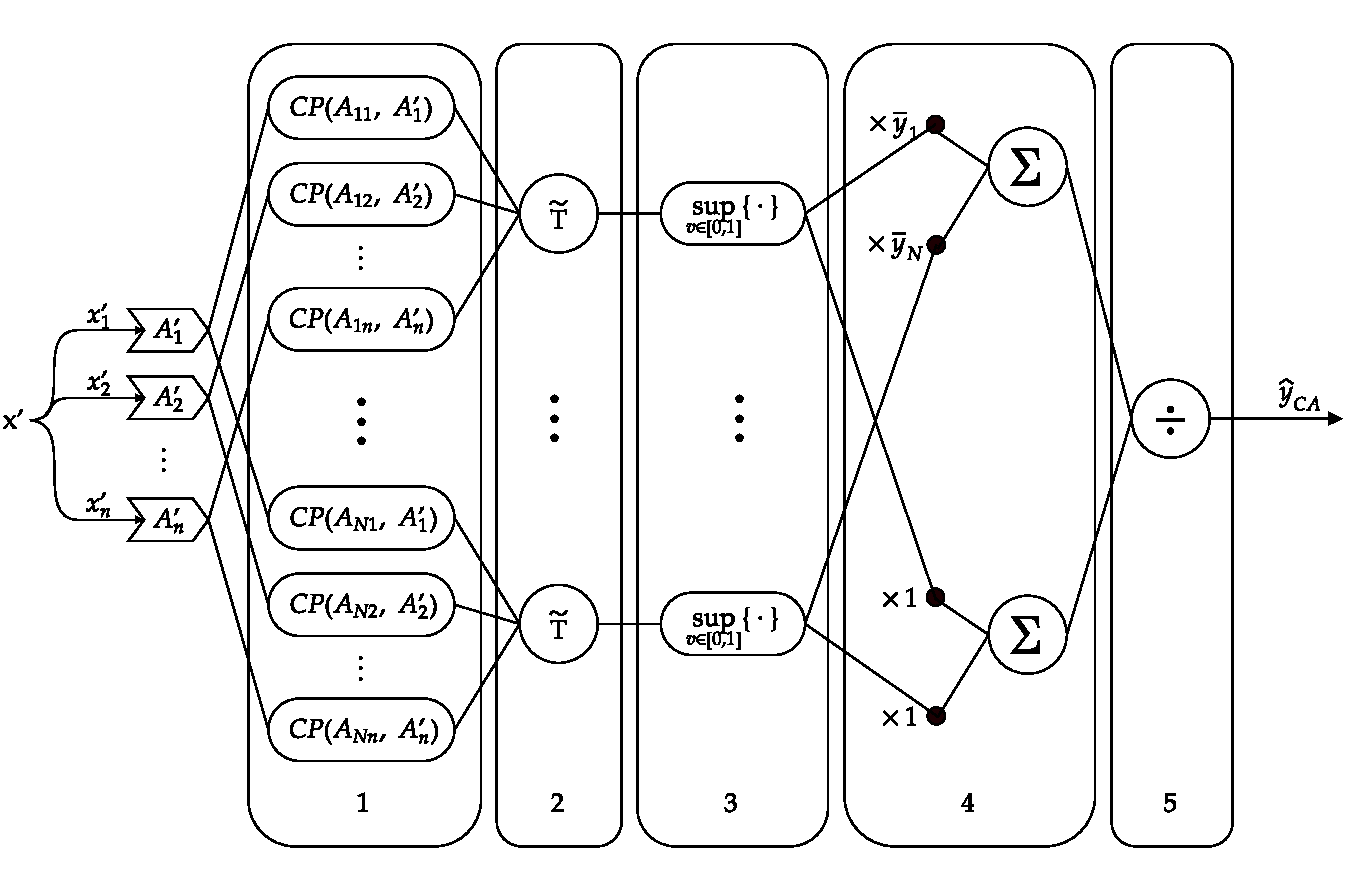
\includegraphics[scale=0.8]{neurofuzzysystem-defuzzification-ca-for-sr-impl}
	\caption{Схема нейро-нечеткой системы с использованием дефаззификации по методу среднего центра для $S$- и $R$-импликаций}
	\label{fig:neurofuzzysystem-defuzzification-ca-for-sr-impl}
\end{figure}

Поскольку $\mu_{B_r}(\overline{y}_k) = 1$ при $k = r$, тогда по формуле (\ref{eqn:ftv-compute-9}) $\mu_{B'_k}(\overline{y}_k)$ выразится:
\begin{align}
	\label{eqn:defuz-ca-3}
	\mu_{B'_k}(\overline{y}_k) &= \sup_{v\in [0, 1]} \left\{\tau_{A_k|A'}\overset{\mathrm{T}_2}{\star} I\left(v, \mu_{B_k}(\overline{y}_k)\right)\right\}\\ &= \sup_{v\in [0, 1]} \left\{\tau_{A_k|A'}\overset{\mathrm{T}_2}{\star} I\left(v, 1\right)\right\}.
\end{align}

Обозначив $I(v, 1) = I_1(v)$, с учетом () формула дефаззификации (\ref{eqn:defuz-ca-3}) примет вид:
\begin{equation}
	\label{eqn:defuz-ca-4}
	\hat{y}_{CA} = \frac{\sum_{k=1}^{N} \bar{y}_k \sup_{v\in [0, 1]} \left\{\tau_{A_r|A'}\overset{\mathrm{T}_2}{\star} I_1(v) \right\}}{\sum_{k=1}^{N} \sup_{v\in [0, 1]} \left\{\tau_{A_r|A'}\overset{\mathrm{T}_2}{\star} I_1(v) \right\}}
\end{equation}

Рассмотрим вычисление $\tau_k$ для различных категорий импликаций:
\begin{itemize}
	\item для \textit{S}-импликаций:
	\begin{align*}
		I_1(v) = I(v, 1) &= S\left\{1-a, 1\right\} = 1\\
	\end{align*}
	\item для \textit{R}-импликаций:
	\begin{align*}
		I_1(v) = I(v, 1) &= \sup_z \left\{z | T(v, z) \le 1\right\}&\quad v\in [0, 1]\\
		&= \sup_z \left\{z | \forall z\right\}&\quad z\in [0, 1]\\
		&= 1
	\end{align*}
	\item для \textit{Q}-импликаций:
	\begin{align*}
		I_1(v) = I(v, 1) &= S\left\{1-v, T(v, 1)\right\}\\
		&= S\left\{1-v, v\right\}\\
	\end{align*}
\end{itemize}


Тогда для \textit{S}- и \textit{R}-импликаций формула (\ref{eqn:defuz-ca-4}) с учетом свойства $t$-нормы $T(a, 1) = a$ примет вид:
\begin{align}
\hat{y}_{CA} &= \frac{\sum_{k=1}^{N} \bar{y}_k \sup_{v\in [0, 1]} \left\{\tau_{\mathbf{A_r}|\mathbf{A'}}\overset{\mathrm{T}_2}{\star} 1 \right\}}{\sum_{k=1}^{N} \sup_{v\in [0, 1]} \left\{\tau_{\mathbf{A_r}|\mathbf{A'}}\overset{\mathrm{T}_2}{\star} 1 \right\}}\\ &= \frac{\sum_{k=1}^{N} \bar{y}_k \sup_{v\in [0, 1]} \left\{\tau_{\mathbf{A_r}|\mathbf{A'}}\right\}}{\sum_{k=1}^{N} \sup_{v\in [0, 1]} \left\{\tau_{\mathbf{A_r}|\mathbf{A'}}\right\}},
\end{align}
а для \textit{Q}-импликации:
\begin{equation}
	\hat{y}_{CA} = \frac{\sum_{k=1}^{N} \bar{y}_k \sup_{v\in [0, 1]} \left\{\tau_{\mathbf{A_r}|\mathbf{A'}}\overset{\mathrm{T}_2}{\star} S\left\{1-v, v\right\} \right\}}{\sum_{k=1}^{N} \sup_{v\in [0, 1]} \left\{\tau_{\mathbf{A_r}|\mathbf{A'}}\overset{\mathrm{T}_2}{\star} S\left\{1-v, v\right\} \right\}}
\end{equation}

Схема нейро-нечеткого системы соответствующая формуле дефаззификации (\ref{}) изображена на рисунке \cref{fig:neurofuzzysystem-defuzzification-ca-for-sr-impl}.

\subsection{Дефаззификация по методу центра тяжести}

(center of gravity)

Если выходное значение блока выработки решения представляет собой единственное агрегированное нечеткое множество $B'$, следует рассмотреть к использованию данный и последующие методы дефаззификации. Этот метод можно сопоставить со схемой вычисления математического ожидания случайной величины при данном ее распределении.

\begin{equation*}
\label{eqn:defuz-cog-1}
\hat{y}_{CoG} = \frac{\int_Y y \mu_{B'}(y) dy}{\int_Y \mu_{B'}(y) dy}
\end{equation*}

Тогда (\ref{}) при использовании данной импликации запишется в виде:
\begin{equation}
\hat{y}_{CoG} = \frac{\int_Y y \Tnorm_{r=1}^N \left\{sup_{v\in [0, 1]} \left\{\tau_{\mathbf{A_r}|\mathbf{A'}}\overset{\mathrm{T}_2}{\star} I\left(v, \mu_{B_r}(y)\right)\right\}\right\} dy}{\int_Y \Tnorm_{r=1}^N \left\{sup_{v\in [0, 1]} \left\{\tau_{\mathbf{A_r}|\mathbf{A'}}\overset{\mathrm{T}_2}{\star} I\left(v, \mu_{B_r}(y)\right)\right\}\right\} dy}
\label{eqn:defuz-cog-2}
\end{equation}

Значение $\hat{y}_{CoG}$ в данном способе дефаззификации может быть вычислено с применением численных методов. Однако существует упрощенная схема нахождения выходного значения в данном методе с помощью дискретной формулы центра тяжести в точках центров функций принадлежности термов выходной лингвистической переменной или ф. п. консеквентов правил в базе правил \cite{rutkovskiy2010}. Эта схема выражается формулой ниже.

\begin{equation}
\label{eqn:defuz-cog-3}
\hat{y}_{CoG} = \frac{\sum_{k=1}^{N} \overline{y}_k \mu_{B'}(\overline{y}_k)}{\sum_{k=1}^{N} \mu_{B'}(\overline{y}_k)},
\end{equation}
где $\overline{y}_k$ --- центр ф. п. нечеткого множества $B_k$, то есть такое значение $y$, в котором $\max_y \mu_{B_k}(y) = 1$.

В этом случае формула (\ref{}) на основе (\ref{}) примет вид:
\begin{align}
	\label{eqn:defuz-cog-4}
	\hat{y}_{CoG} = \frac{\sum_{k=1}^{N} \overline{y}_k \Tnorm_{r=1}^N \left\{sup_{v\in [0, 1]} \left\{\tau_{\mathbf{A_r}|\mathbf{A'}}\overset{\mathrm{T}_2}{\star} I\left(v, \mu_{B_r}(\overline{y}_k)\right)\right\}\right\}}{\sum_{k=1}^{N} \Tnorm_{r=1}^N \left\{sup_{v\in [0, 1]} \left\{\tau_{\mathbf{A_r}|\mathbf{A'}}\overset{\mathrm{T}_2}{\star} I\left(v, \mu_{B_r}(\overline{y}_k)\right)\right\}\right\}},
\end{align}

Выражение внутри фигурных скобок оператора $\sup_{v\in [0, 1]}\{\cdot\}$, представляющее композицию двух нечетких множеств на пространстве истинности, есть определение \textit{возможности}, то есть соответствие того, что $\tau_{\mathbf{A_r}|\mathbf{A'}}$ есть $\tau_{k\,r}$ и наоборот. Обозначим величину возможности:
\begin{equation}
	\sup_{v\in [0,1]}\left\{\tau_{\mathbf{A_r}|\mathbf{A'}}\overset{\mathrm{T}_2}{\star}\tau_{k\,r}\right\} = \Pi_{k\,r}
\end{equation}

Поскольку импликация в выражении (\ref(eqn:defuz-cog-4)) не зависит от входных данных, то значения $I(v, \mu_{B_r}(\overline{y}_k)) = \tau_{k\,r}, k=\overline{1,N}, r=\overline{1,N}$ могут быть вычислены предварительно, то есть до использования композиционного правила вывода.


\begin{figure}[ht]
	\centering
	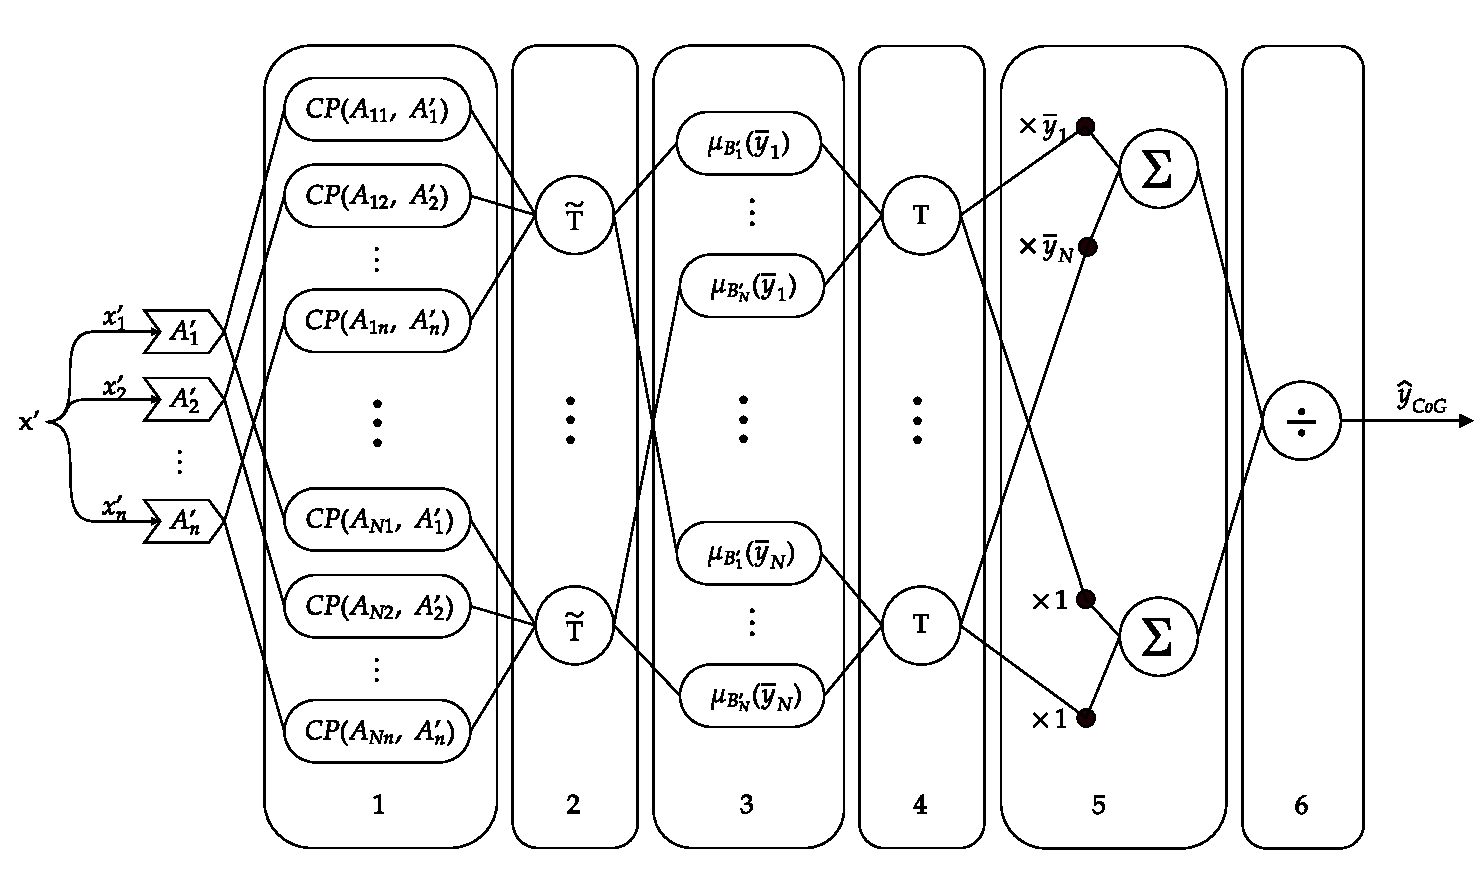
\includegraphics[scale=0.7]{neurofuzzysystem-defuzzification-cog}
	\caption{Схема нейро-нечеткой системы с использованием дефаззификации по методу центра тяжести}
	\label{fig:neurofuzzysystem-defuzzification-cog}
\end{figure}


\begin{figure}[ht]
	\centering
	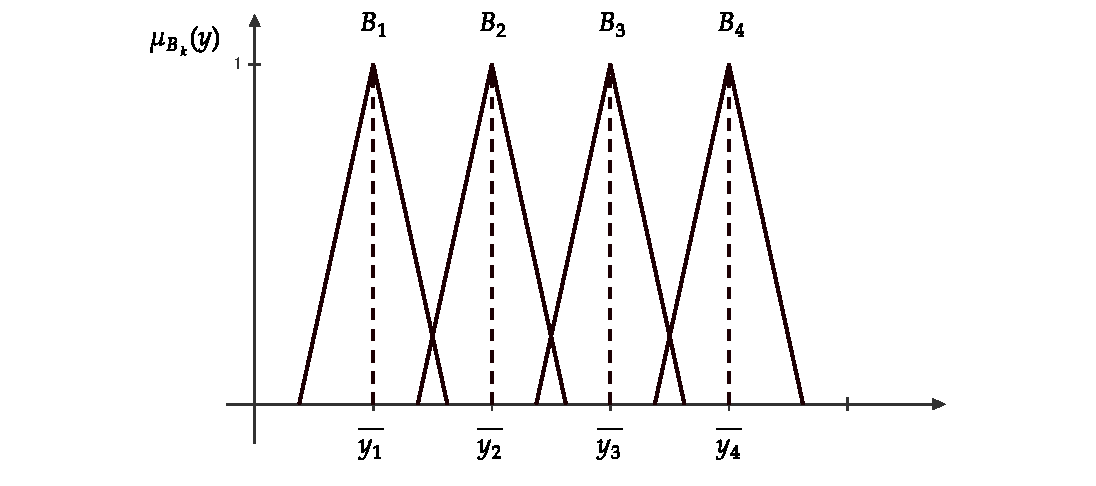
\includegraphics[]{out-mf-with-low-crossing}
	\caption{Пример нечетких множеств, удовлетворяющих условию $\mu_{B_k}(y_r) = 0$ для $y \ne r$}
	\label{fig:out_mf_with_low_crossing}
\end{figure}

Одна из возможностей упрощения процедуры вывода возникает, когда функции принадлежностей термов выходной лингвистической переменной достаточно удалены друг от друга и имеют низкую степень взаимного пересечения, то есть выполняется соотношение $\mu_{B_k}(y_r) \approx 0$ при $k \ne r$, что проиллюстрировано на рисунке \cref{fig:out_mf_with_low_crossing}.

Рассмотрим вычисление $\tau_{k\,r}$ для различных категорий импликаций:
\begin{itemize}
	\item для \textit{S}-импликации
	\begin{equation*}
		\tau_{k\,r}(v) = \begin{cases}
			1-v, & \quad \text{если } k \ne r \\
			1, & \quad \text{если } k = r
		\end{cases}
	\end{equation*}
	\begin{equation*}
		\hat{y}_{CoG} = \frac{\sum_{k=1}^{N} \overline{y}_k \Tnorm_{r=1}^N \left\{sup_{v\in [0, 1]} \left\{\tau_{A_r|A'}\overset{\mathrm{T}_2}{\star}(1-v)\right\}\right\}}{\sum_{k=1}^{N} \Tnorm_{r=1}^N \left\{sup_{v\in [0, 1]} \left\{\tau_{A_r|A'}\overset{\mathrm{T}_2}{\star}(1-v)\right\}\right\}},
	\end{equation*}
	\item для \textit{R}-импликации
	\begin{equation*}
	\tau_{k\,r}(v) = \begin{cases}
		\delta(v), & \text{если } k \ne r \\
		1, & \text{если } k = r
	\end{cases},
	\quad\text{где }
	\delta(v) = \begin{cases}
		1, & v = 0 \\
		0, & v > 0
	\end{cases}
	\end{equation*}
	\begin{equation*}
	\hat{y}_{CoG} = \frac{\sum_{k=1}^{N} \overline{y}_k \Tnorm_{r=1}^N \left\{\tau_{A_r|A'}(0)\right\}}{\sum_{k=1}^{N} \Tnorm_{r=1}^N \left\{\tau_{A_r|A'}(0)\right\}},
	\end{equation*}
	\item для \textit{S}-импликации
	\begin{equation*}
	\tau_{k\,r}(v) = \begin{cases}
		1-v, & \quad \text{если } k \ne r \\
		max(1-v, v), & \quad \text{если } k = r
	\end{cases}
	\end{equation*}
	\begin{equation*}
	\hat{y}_{CoG} = \frac{
		\sum_{k=1}^{N} \overline{y}_k \mathrm{T}_2 \left\{
			sup_{v\in [0, 1]} \left\{\tau_{A_k|A'}\overset{\mathrm{T}_2}{\star}max(1-v, v)\right\}
			\Tnorm_{\substack{r=1\\r\ne k}}^N \left\{
				sup_{v\in [0, 1]} \left\{\tau_{A_r|A'}\overset{\mathrm{T}_2}{\star}(1-v)\right\}
			\right\}
		\right\}
	}{
		\sum_{k=1}^{N} \mathrm{T}_2 \left\{
			sup_{v\in [0, 1]} \left\{\tau_{A_k|A'}\overset{\mathrm{T}_2}{\star}max(1-v, v)\right\}
			\Tnorm_{\substack{r=1\\r\ne k}}^N \left\{
				sup_{v\in [0, 1]} \left\{\tau_{A_r|A'}\overset{\mathrm{T}_2}{\star}(1-v)\right\}
			\right\}
		\right\}
	},
	\end{equation*}
\end{itemize}

\todo{Можно организовать вычисление всех значений $b_{k\,r}$ $\tau_{k\,r}$, но использовать разреженные матрицы в качестве структуры данных для хранения значений где $b_{k\,r} > 0$.}

\todo{Приведенные выклладки справедливы не только для функций принадлежностей отдельных термов, а и для набора кластеризованных в небольшие группы функций принадлжености со значительной степенью пересечения. При такой конфигурации выходного нечеткого пространства нет необходимости включать в процесс вывода правила, в которых функции принадлжености консеквента имеют низкий уровень пересечения с ф. п. правил, имеющих высокий уровень срабатывания для данного входа нечеткой системы.}

\subsection{Дефаззификация по методу центра области}

(center of area)

Данный метод можно сопоставить со схемой вычисления медианы случайной величины при заданном ее распределении. Формула вычисления дефаззифицированного значения $y^*_{CoA}$ имеет вид:

\begin{equation*}
\int_{\inf Y}^{\hat{y}_{CoA}} \mu_{B'}(y) dy = \int_{\hat{y}_{CoA}}^{\sup Y} \mu_{B'}(y) dy
\end{equation*}

\begin{align*}
\int_{\inf Y}^{\hat{y}_{CoA}} \Tnorm_{r=1}^N \left\{\sup_{v\in [0, 1]} \left\{\tau_{A_r|A'}\overset{\mathrm{T}_2}{\star} I\left(v, \mu_{B_r}(y)\right)\right\}\right\} dy =\\
= \int_{\hat{y}_{CoA}}^{\sup Y} \Tnorm_{r=1}^N \left\{\sup_{v\in [0, 1]} \left\{\tau_{A_r|A'}\overset{\mathrm{T}_2}{\star} I\left(v, \mu_{B_r}(y)\right)\right\}\right\} dy
\end{align*}

\subsection{Дефаззификация по методу среднего максимума}

\begin{equation*}
\hat{y}_{MeOM} = \frac{\sum_{x \in core(B')} x}{|core(B')|},
\end{equation*}
где $core(B') = \left\{y | y \in Y \textrm{ and } \mu_{B'}(y) = \sup_{y' \in Y} \mu_{B'}(y')\right\}$. 

Данный метод аналогичен по схеме вычисления моде случайной величины при заданном ее распределении. В случае унимодального вида функции принадлежности $\mu_{B'}(y)$ данный способ дефаззификации можно упростить до метода максимума функции принадлежности:
\[
\hat{y}_{MeOM} = \mathrm{arg\,max}_{y \in Y} \mu_{B'}(y).
\]

Тогда 
\begin{equation}
	\hat{y}_{MeOM} = \arg\,\max_{y\in Y} \Tnorm_{r=1}^N \left\{\sup_{v\in [0, 1]} \left\{\tau_{A_r|A'}\overset{\mathrm{T}_2}{\star} I\left(v, \mu_{B_r}(y)\right)\right\}\right\}
\end{equation}


\section{Классификация объектов на основе нечеткого вывода с использованием нечеткого значения истинности}

Описанная в разделе \cref{sec:ch2/ftv-based-inference-statement} нечеткая система в общем случае используется для моделирования. Тогда, можно использовать этот логический вывод для определения принадлежности некоторого объекта к каждому из заданного множества классов, т. е. с помощью этой нечеткой системы можно решать задачу многоклассовой классификации.

В классических методах классификация производится для данного объекта $q$ с набором значений атрибутов, каждый из которых формализуется числовым значением признака. В случае использовании для этого нечеткой системы, значения признаков формализуются посредством термов лингвистических переменных $\mathbf{x}=[x_1,\dots,x_n ]$, совокупность значений которых формирует вектор $\mathbf{A'}=\left[A'_1,A'_2,\dots,A'_n\right]$, что соответствует посылке:
\begin{equation*}
	\langle x_1\text{ есть }A'_1\text{ и }x_2\text{ есть }A'_2\text{ и }\dots \text{ и }x_n\text{ есть }A'_n\rangle
\end{equation*}

При этом рассмотренный выше метод нечеткого вывода позволяет обрабатывать значения признаков объекта, заданные с использованием фаззификации типа non-singleton, учитывающей зашумленность значений этих признаков.

%Например, значение лингвистической переменной может быть задано нечетким множеством, характеризующегося гауссовой функцией принадлежности. В этой функции значение мат ожидания равно значению признака объекта, а среднеквадратичное отклонение – совпадает с среднеквадратичным отклонением всего набора объектов, принадлежащих данному классу.

Пусть классификация производится для множества из $m$ классов $\Omega=\left\{\omega_1,\dots,\omega_m\right\}$. Тогда база знаний нечеткой систем описывается набором из $N$ правил вида:

\begin{equation}
	\begin{aligned}
	R_k: \textrm{Если }&x_1\textrm{ есть }A_{k1}\textrm{ и }x_2\textrm{ есть }A_{k2}\textrm{ и }\dots\textrm{ и } x_n\textrm{ есть }A_{kn},&\\
	\textrm{ то }&q_k \in \omega_1 (\bar{z}_{k1})\textrm{ и }q_k \in \omega_2 (\bar{z}_{k2})\textrm{ и }\dots\textrm{ и }q_k \in \omega_m (\bar{z}_{km}), k \in \overline{1,N},
	\end{aligned}
	\label{eqn:fuzzy-classify-1}
\end{equation}

где $z_{kj}$ --- степень принадлежности объекта $q$ к классу $\omega_j$ в соответствии с правилом $R_k$. Значения $\bar{z}_{kj}$ могут быть определены при помощи метода парных сравнений \cite{} на основании набора объектов-образцов $Q = \left\{q_k\right\}_{k=1}^N$. Каждому значению $z_{kj}$ можно поставить в соответствие значение лингвистической переменной $z_j$, которое выражается нечетким множеством $B_{kj}$ имеющим в качестве базового множеств диапазон $[0, 1]$, обозначающий вероятность принадлежности объекта к $j$-му классу.

В случае, если база правил представляет собой набор эталонных объектов процедура нечеткого вывода может быть упрощена за счет использования в качестве термов выходных лингвистических переменных синглтонных нечетких множеств $B_{k1}, B_{k2}, \dots, B_{km}$ c функцией принадлежности:
\begin{equation*}
	\mu_{B_{kj}}(z_j) = \begin{cases}
		1, \quad&\text{если } z_j = \bar{z}_{kj},\\
		0, \quad&\text{если } z_j \ne \bar{z}_{kj}.
	\end{cases}
\end{equation*}	

Тогда, согласно (\ref{}):
\begin{equation*}
	1
\end{equation*}

Принадлежность объекта к одному из $m$ классов затем определяется по формуле:
\[
	j^* = \argmax_{j=\overline{1,m}} \hat{z}_j,
\]
где $\hat{z}_j$ --- дефаззифицированное значение выходной лингвистической переменной $z_j$.

Если задача мультиклассовой классификации позволяет отнесение объекта сразу к нескольким классам, окончательное решение может быть получено на основании условий:
\begin{equation*}
	\begin{cases}
		q \in \omega_j, \quad&\text{если }\hat{z}_j \geq z_{inc},\\
		q \notin \omega_j, \quad&\text{если }\hat{z}_j \leq z_{exc},\\
		\text{не определено}, \quad&\text{если }z_{exc} < \hat{z}_j < z_{inc},
	\end{cases}
\end{equation*}
где числа $z_{inc}$ и $z_{exc}$ --- фиксированные пороговые значения, такие, что:
\[
	0 \leq z_{exc} \leq z_{inc} \leq 1.
\]

%В этом правиле степень принадлежности объекта $q$ к классу $\omega_j$ задается  значением $(z_{kj})$, которому можно поставить в соответствие значение лингвистической переменной $z_j$. Это значение выражается нечетким множеством имеющим в качестве базового множеств диапазон $[0,1]$ вероятности принадлежности объекта к заданному классу.

%Тогда, правило \ref{eqn:fuzzy-classify-1} можно переписать в виде, в котором было записано правило (1) для системы нечеткого вывода, заменив при этом лингвистические переменные y_j на z_j, где j=(1,m) ̅.
%R_k:Если x_1  есть A_1k  и x_2  есть A_2k  и,…,и x_n  есть A_nk,
%то z_1  есть B_1k  и z_2  есть B_2k  и… и z_m  есть B_mk.


\section{Прогнозирование временных рядов на основе нечетких систем логического типа с использованием нечеткого значения истинности}

Определив НЗИ $CP(\mathbf{A_{k}, \mathbf{A'}})$ для антецедента правила $R_k$ согласно (\ref{eqn:ftv-compute-12}) и (\ref{eqn:ftv-compute-8}), можно переписать правило $R_k$ в виде:
\begin{align*}
	R_k: \textrm{Если }&CP(\mathbf{A_{k}, \mathbf{A'}}),&\\
	\textrm{ то }&y_{t+1}\textrm{ есть }A_{k\,p+1},&k\in\overline{1,N}.
\end{align*}

\todo{Вычисленное значение истинности для каждого правила выражает соответствие среза измерений порождаемых некоторым величины некоторой единице знаний о динамике этого процесса.}

Если используется логический метод вывода на основе дефаззификации по центру тяжести, то согласно (\ref{}) нечеткий вывод выражается:
\begin{equation}
\hat{y}_{t+1} = \frac{\int_Y y_{t+1} \underset{k=\overline{1,N}}{\textrm{T}}\Biggl\{\sup_{v \in [0,1]}\biggl\{\tau_{\mathbf{A_k}|\mathbf{A'}}(v)\overset{T_2}{\star} I(v, \mu_{A_{k\,p+1}}(y_{t+1}))\biggr\}\Biggr\} dy_{t+1}}{\int_Y \underset{k=\overline{1,N}}{\textrm{T}}\Biggl\{\sup_{v \in [0,1]}\biggl\{\tau_{\mathbf{A_k}|\mathbf{A'}}(v)\overset{T_2}{\star} I(v, \mu_{A_{k\,p+1}}(y_{t+1}))\biggr\}\Biggr\} dy_{t+1}}
\end{equation}



\section{Выводы}

\begin{enumerate}
	\item С использованием нечеткого значения истинности можно построить альтернативный метод нечеткого логического вывода. Данный метод соответствует каноническому логическому выводу Заде за счет эквивалентного преобразования пространства антецедента правил. Преобразование истинностной модификации отображает многомерное пространство антецедента в одномерное пространство истинности, из-за чего база правил приобретает новую структуру правил вида: <<Если \textit{истинно}, то $B_k$>>. Вычисление посылки нечеткого значения истинности составляет предшествующий непосредственно логическому выводу этап, и формируется из нахождения НЗИ между нечетким множеством в антецеденте и входной посылки по каждому входу отдельно и последующей свертки в единое пространство НЗИ с помощью расширенной $t$-нормы --- $\tilde{\mathrm{T}}$.
	\item Для предложенного метода нечеткого вывода применимы различные способы дефаззификации выходного значения. \todo{Схема вычисления дефаззификации по методу среднего центра значительно упрощается. Вычисление дефаззификации по упрощенной схеме сводится к нахождению величины меры возможности $1$. В случае, когда нечеткие множества удалены друг от дурга и имеют низкую степень взаимного пересечения итоговые формулы дефаззификации упрощаются за счет. Это позволяет\dots}
	\item Показано как \dots применен для решения задач классификации объектов с нечеткими атрибутами и для прогнозирования временных рядов.
\end{enumerate}

\todo{Проведен анализ\dots}

В главе приведены итоговые формулы нечеткого вывода на основе нечеткого значения истинности для различных методов дефаззификации. Также выведены упрощенные формулы вычисления дефаззифицированного значения для различных специальных категорий импликаций.

Дано формальное описание применения разработанной модели нечеткого логического вывода в задаче прогнозирования временных рядов. Приведены существующие подходы фаззификации значений временных рядов и методы автоматического подбора параметров термов лингвистической переменной и формирования базы правил на основе наборов обучающих данных.

\FloatBarrier
